\documentclass[submit]{harvardml}

% FDV: Make sure all front matter has correct years, dates, book sections, etc.
\course{CS181-S23}
\assignment{Assignment \#2}
\duedate{11:59pm EST, Feb 23th, 2023}
\usepackage[OT1]{fontenc}
\usepackage[colorlinks,citecolor=blue,urlcolor=blue]{hyperref}
\usepackage[pdftex]{graphicx}
\usepackage{subfig}
\usepackage{fullpage}
\usepackage{amsmath}
\usepackage{amssymb}
\usepackage{framed}
\usepackage{color}
\usepackage{soul}
\usepackage{todonotes}
\usepackage{listings}
\usepackage{common}
\usepackage{enumitem}
\usepackage{bm}
\usepackage{bbm}
\newcommand{\B}{\text{B}}
\newcommand{\Beta}{\text{Beta}}

\usepackage[mmddyyyy,hhmmss]{datetime}

\definecolor{verbgray}{gray}{0.9}

\lstnewenvironment{csv}{%
  \lstset{backgroundcolor=\color{verbgray},
  frame=single,
  framerule=0pt,
  basicstyle=\ttfamily,
  columns=fullflexible}}{}

\begin{document}

\begin{center}
{\Large Homework 2: Classification and Bias-Variance Trade-offs}\\
\end{center}

\subsection*{Introduction}

This homework is about classification, bias-variance trade-offs, and uncertainty quantification. In lecture we have primarily focused on binary classifiers trained to discriminate between two classes. In multiclass classification, we
discriminate between three or more classes. 
We encourage you to read
CS181 Textbook's Chapter 3 for more information on linear
classification, gradient descent, and classification in the discriminative setting. Read Chapter 2.8 for more
information on the trade-offs between bias and variance.

The datasets that we will be working with relate to astronomical observations. The first dataset, found at \verb|data/planet-obs.csv|, contains information on whether a planet was observed (as a binary variable) at given points in time. This will be used in Problem 1. The second dataset, available at \verb|data/hr.csv|, details different kinds of stars and their measured magnitude and temperature. You will work with this data in Problem 3.
As a general note, for classification problems we imagine that we have
the input matrix $\boldX \in \reals^{n \times d}$ (or perhaps they
have been mapped to some basis $\bm{\Phi}$, without loss of
generality) with outputs now ``one-hot encoded."  This means that if
there are~$K$ output classes, rather than representing the output
label $y$ as an integer~${1,2,\ldots,K}$, we represent $\boldy$ as a
``one-hot" vector of length~$K$. A ``one-hot" vector is defined as
having every component equal to 0 except for a single component which
has value equal to 1.  For example, if there are $K = 7$ classes and a
particular data point belongs to class 3, then the target vector for
this data point would be~$\boldy = [0,0,1,0,0,0,0]$.  We will define
$C_1$ to be the one-hot vector for the 1st class, $C_2$ for the 2nd
class, etc.  Thus, in the previous example $\boldy = C_3$. If there
are $K$ total classes, then the set of possible labels is $\{C_1
\ldots C_K \} = \{C_k\}_{k=1}^K$.  Throughout the assignment we will
assume that each label $\boldy \in \{C_k\}_{k=1}^K$ unless otherwise
specified. The most common exception is the case of binary classification
($K = 2$), in which case labels are the typical integers $y \in \{0, 1\}$.

In problems 1 and 3, you may use \texttt{numpy} or \texttt{scipy}, but
not \texttt{scipy.optimize} or \texttt{sklearn}. Example code given is
in Python 3.

Please type your solutions after the corresponding problems using this
\LaTeX\ template, and start each problem on a new page.

Please submit the \textbf{writeup PDF to the Gradescope assignment `HW2'}. Remember to assign pages for each question.  \textbf{You must include your plots in your writeup PDF. } The supplemental files will only be checked in special cases, e.g. honor code issues, etc.

Please submit your \textbf{\LaTeX\ file and code files to the Gradescope assignment `HW2 - Supplemental'}. 

%%%%%%%%%%%%%%%%%%%%%%%%%%%%%%%%%%%%%%%%%%%%%
% Problem 1
%%%%%%%%%%%%%%%%%%%%%%%%%%%%%%%%%%%%%%%%%%%%%

\begin{problem}[Exploring Bias-Variance and Uncertainty]
In this problem, we will explore the bias and variance of a few different model classes when it comes to logistic regression and investigate two sources of predictive uncertainty.

We are currently managing a powerful telescope that is being used to monitor and gather measurements of some planet of interest. At certain times however, our telescope is unable to detect the planet at all. The data in \verb|data/planet-obs.csv| records the observation time in the ``Time" column and whether the planet was detected in the ``Observed" column (with the value 1 representing that it was observed). Since it is expensive to use and maintain the telescope, we would like to build a model to help us schedule and find times when we are likely to detect the planet.

\begin{enumerate}

\item First split the data into 10 mini-datasets of size $N = 30$ (i.e. dataset 1 consists of the first 30 observations, dataset 2 consists of the next 30, etc. This has already been done for you). Consider the three bases $\boldsymbol\phi_1(t) = [1, t]$, $\boldsymbol\phi_2(t) = [1,
  t, t^2]$, and $\boldsymbol\phi_3(t) = [1, t, t^2, t^3, t^4, t^5]$. For each of these bases, fit a logistic regression model using sigmoid($\boldw^\top \boldsymbol\phi(t)$) to each dataset by using gradient descent to
  minimize the negative log-likelihood.  This means you will be
  running gradient descent 10 times for each basis, once for each
  dataset.
  
  Use the given starting values of $\boldw$ and a learning rate of $\eta=0.001$, take 10,000 update
  steps for each gradient descent run, and make sure to average the
  gradient over the data points at each step. These parameters,
  while not perfect, will ensure your code runs reasonably quickly. 

\item After consulting with a domain expert, we find that the probability of observing the planet is periodic as the planet revolves around its star---we are more likely to observe the planet when it is in front of its star than when it is behind it. In fact, the expert determines that observation follows the generating process $y \sim \text{Bern}(f(t))$, where $f(t) = 0.4 \times \cos(1.1t + 1) + 0.5$ for $t \in [0, 6]$ and $y \in \{0,1\}$. Note that we, the modelers, do not usually see the true data distribution. Knowledge of the true $f(t)$ is only exposed in this problem to allow for verification of the true bias.

Use the given code to plot the true process versus your learned models. Include your plots in your solution PDF.

\textbf{In no more than 5 sentences}, explain how bias and variance reflected in the 3 types of curves on the graphs.  How do the fits of the individual and mean prediction functions change?  Keeping in mind that none of the model classes match the true generating process exactly, discuss the extent to which each of the bases approximates the true process.

\item If we were to increase the size of each dataset drawn from $N = 30$ to a larger number, how would the bias and variance change for each basis? Why might this be the case? You may experiment with generating your own data that follows the true process and plotting the results, but this is \textbf{not} necessary. \textbf{Your response should not be longer than 5 sentences}.

\item Consider the test point $t = 0.1$. Using your models trained on basis $\boldsymbol\phi_3$, report the predicted probability of observation of the \textit{first} model (the model trained on the first 30 data points). How can we interpret this probability as a measure of uncertainty? Then, compute the variance of the classification probability over your 10 models at the same point $t = 0.1$. How does this measurement capture another source of uncertainty, and how does this differ from the uncertainty represented by the classification probability?

Repeat this process (reporting the first model's classification probability and the variance over the 10 models) for the point $t = 3.2$. At which point in time would you be more confident in detecting the planet? There's no right answer---you should consider the two different types of uncertainty and their implications when translating from model output to decision making.

\end{enumerate}
\end{problem}
 \let\cleardoublepage\clearpage
\pagebreak
 \textbf{Problem 1 Solution:}\\
 \begin{enumerate}
     \item Solution included in my code file \\
     \item\\
     Here are my three graphs:\\
     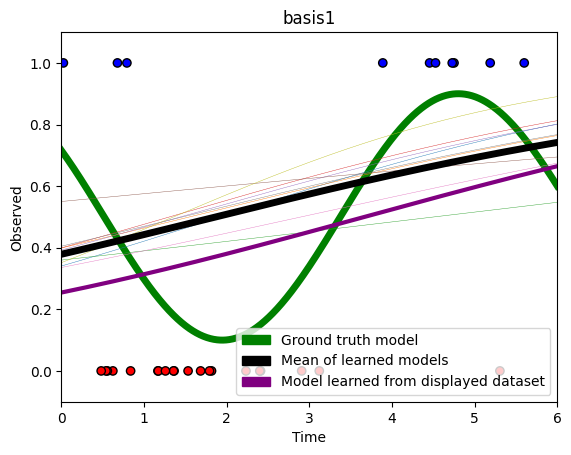
\includegraphics[scale=0.4]{hw2/images/q1_basis1.png}
     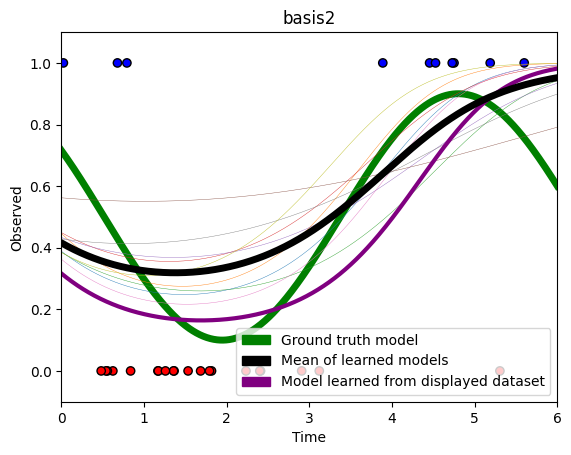
\includegraphics[scale=0.4]{hw2/images/q1_basis2.png}\\
     \begin{center}
         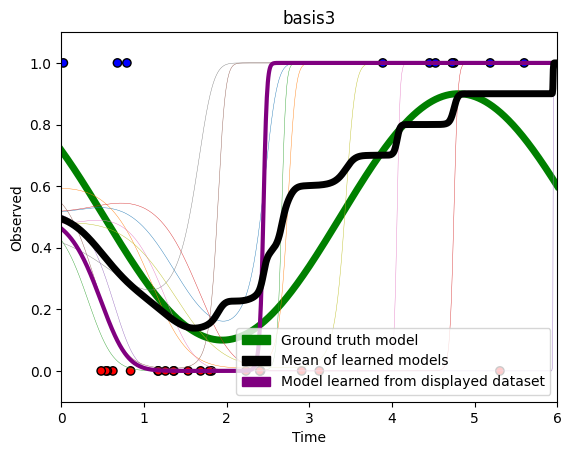
\includegraphics[scale=0.4]{hw2/images/q1_basis3.png}\\
     \end{center}
     From these three plots we can see a general trend that as the polynomial degree of the function increases (as we increase the basis from 1 to 3), the variance of our model increases and the bias decreases. We can see that in the plot for basis 1, our model does not fit the ground truth model very well as it is clearly underfitting the data (a sign of high bias). Furthermore, we can see a low variance because all of the individual models seem pretty similar. On the other hand, the plot for basis 3 seems to be overfitting the data which indicates there is a lower bias and each of the individual models seems very different which is an indication of a high variance. Overall, it seems as though basis 1 does not approximate the true process well, bases 2 begins to approximate the process, and basis 3 does the best job. \\
     
     \item
     Pasted below are 3 plots that display the output when we train our model on 2 datasets of size $N=150$. \\
     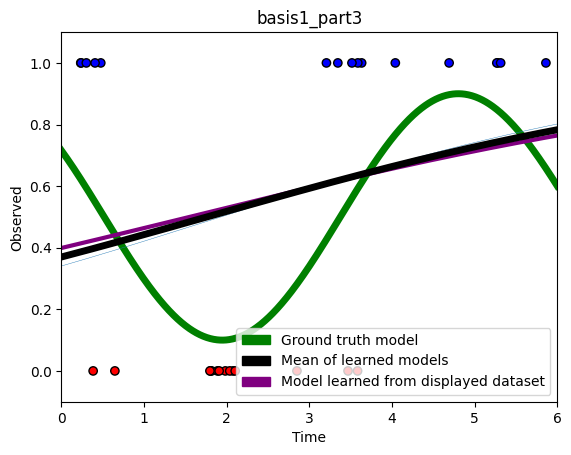
\includegraphics[scale = 0.25]{hw2/images/1.3_basis1.png}
     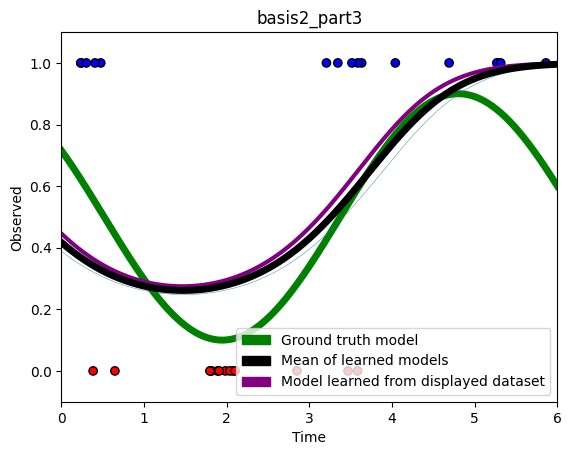
\includegraphics[scale = 0.25]{hw2/images/1.3_basis2.png}
     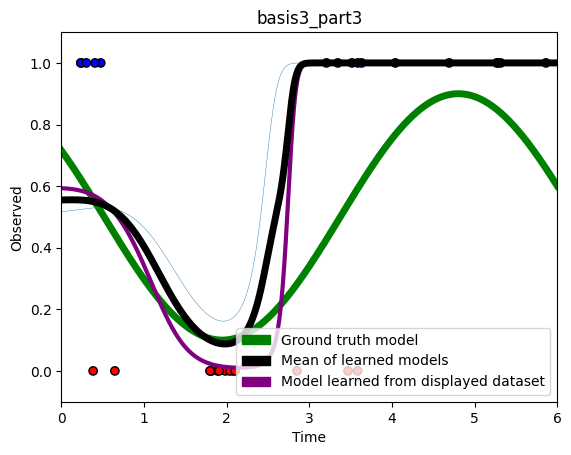
\includegraphics[scale = 0.25]{hw2/images/1.3_basis3.png}\\
     As we can see, if we were to increase the size of each data set then our variance decreases. This is the case because if we have a much larger data set, then a few noisy points would have less of an impact on our model (if we only have a few points then we take into account the noise from each point a lot more) so we would overfit the data less. This is true for all of our bases; however, we know that the less complex bases (basis 1) will have the smallest decrease in variance because it is such a simple model and already has a low variance. Additionally, because it is such a simple model, the bias will basically stay the same because even with more data points it could not fit to the data well enough. Similarly, basis 2 would have a decrease in variance but the bias would most likely stay the same or maybe increase a tiny bit. Basis 3 will feel the decrease in variance the most because it is the most complex of the models and the bias would also most likely stay the same or slightly increase.\\ 
     \item
     \textbf{Test point $t=0.1$:}\\
     Predicted probability of observation of first model = $0.5198107803372445$\\
     \\
     We can interpret this probability as a measure of our uncertainty about the classification of our data. This probability is not equal to 1 or 0 which indicates we are not positive that it should be classified as class 1 or class 2. This probability is really close to $0.5$ which means we are pretty uncertain about the class.\\
     \\
     Variance = $0.0033896231687377586$\\
     This measurement captures another source of uncertainty because it indicates that each of our models may have a different predicted probability of observation for this test data point. This variance is telling us how much our models differ in their predictions - so if they differ more then we are more uncertain. A high variance indicates a high level of uncertainty.\\
     \\ 
    \textbf{Test point $t=3.2$:}\\
    Predicted probability of observation of first model = $0.9999999998523916$\\
    Variance = $0.23282232401975583$\\
    \\
    Even though the predicted probability of observation is a lot more clearly pointing to a particular class at $t=3.2$, I would be more confident detecting my planet at $t=0.1$ because the variance is so so much smaller than the variance at time $t=3.2$. This drastic difference indicates that the models differ significantly more at $t=3.2$ which is why I would be less confident then.\\

     
 \end{enumerate}

%%%%%%%%%%%%%%%%%%%%%%%%%%%%%%%%%%%%%%%%%%%%%
% Problem 2
%%%%%%%%%%%%%%%%%%%%%%%%%%%%%%%%%%%%%%%%%%%%%

\begin{problem}[Multi-class Logistic Regression and Softmax]
The objective of this problem is to generalize binary logistic regression into the more general case of three or more classes. You will use the results of this problem to implement a classifier in Problem 3.

Consider a $K$-class model with $K \geq 3$. Suppose we have a data set $\{(\boldx_i,
\boldy_i)\}_{i=1}^n$ with features $\{\boldx_n\}_{n = 1}^N \in \mathbb{R}^d$ and one-hot encoded outputs $\{\boldy_n\}_{n = 1}^N \in \mathbb{R}^K$ (see the introduction of this homework). For a $K$-dimensional vector $\boldz = [z_1, \dots, z_K]^\top$, define the \textit{softmax} function to be
$$
\text{softmax}(\boldz) = \frac{1}{\sum_{i = 1}^K \exp(z_i)}
\begin{bmatrix}
\exp(z_1) \\
\exp(z_2) \\
\vdots \\
\exp(z_K)
\end{bmatrix}.
$$
In other words, the softmax function is a function from $\mathbb{R}^K$ to $\mathbb{R}^K$ with $k$-th component of the output
$$
\text{softmax}_k(\boldz) = \frac{\exp(z_k)}{\sum_{i = 1}^K \exp(z_i)}.
$$
We will use the shorthand notation $s_k(\boldz)$ to abbreviate the above. Note that the softmax function is the general form of the sigmoid function in binary logistic regression. This means that the derivations in this problem will be very similar to what you have seen in class.

\begin{enumerate}
  \item For $j, k \in \{1, \dots, K\}$, show that the partial derivatives of the softmax function can be written in terms of the softmax function itself in the following form:
  $$
  \frac{\partial s_k(\boldz)}{\partial z_j} = s_k(\boldz)(\delta_{jk} - s_j(\boldz))
  $$
  Here, $\delta_{jk}$ denotes the \textit{Kronecker delta} function $\delta_{jk}$:
  $$
  \delta_{jk} = 
  \begin{cases}
    1 \text{ if } j = k, \\
    0 \text{ if } j \neq k.
  \end{cases}
  $$
  Since all of these partial derivatives are with respect to scalars, you can use the typical quotient rule from your univariate calculus class. It may help to consider the cases $j = k$ and $j \neq k$ separately.
  
  Using the answer above, find the logarithmic derivatives of $\text{softmax}(\boldz)$; that is, find $\displaystyle \frac{\partial \ln s_k(\boldz)}{\partial z_j}$ for $j, k \in \{1, \dots, K\}$.
\end{enumerate}

Multi-class logistic regression has weights $\{\boldw_j\}_{j=1}^K \in \mathbb{R}^d$ for each class, which are often condensed into a single matrix $\boldW \in \mathbb{R}^{K \times d}$ (the $j$-th row of $\boldW$ corresponds to $\boldw_j$). We model the probabilities of class membership independently as
$$
p(\boldy_n = C_k | \boldx_n, \boldW) = s_k(\boldW\boldx_n)
$$
for $k \in \{1, \dots, K\}$ and $n \in \{1, \dots, N\}$.
In addition, let $y_{nk}$ denote the $k$-th component of the output vector $\boldy_n$. 
\begin{enumerate}
    \item[2.] Write out the negative log-likelihood of the data set, $\ell(\boldW) = -\ln p(\{\boldy_n\}_{n=1}^N | \{\boldx_n\}_{n=1}^N, \boldW)$, in terms of $s_k, \boldW, \{\boldx_n\}_{n=1}^N$, and $y_{nk}$. You can start by noting that for a single observation $(\boldx_n, \boldy_n)$,
    $$
    p(\boldy_n | \boldx_n, \boldW) = \prod_{k=1}^Kp(\boldy_n = C_k | \boldx_n, \boldW)^{y_{nk}}
    $$
    because $y_{nk} = 1$ if $\boldy_n$ belongs to class $C_k$ and $y_{nk} = 0$ otherwise. The equation above simply lets us combine all possible class memberships of $\boldy_i$ into a single expression. This is also known as the ``power trick" as we express the probability as a product of terms raised to a power that is either 0 or 1.
\end{enumerate}
\end{problem}

\begin{framed}
\noindent\textbf{Problem 2} (cont.)\\
\begin{enumerate}
    \item[3.] Consider the weight matrix $\boldW$ and the $i$-th feature vector $\boldx_i$. Denote their product as $\boldz_i = \boldW\boldx_i$. Compute the derivative of $\ell(\boldW)$ with respect to the $j$-th coordinate of the $K$-dimensional vector $\boldz_i$ (denoted as $z_{ij}$). In particular, show that 
    $$
    \frac{\partial \ell}{\partial z_{ij}} = \sum_{k = 1}^K y_{ik}(s_j(\boldz_i) - \delta_{kj})
    $$
    You may want to use your answer from part 1. Then, show that the above sum can be simplified:
    $$
    \sum_{k = 1}^K y_{ik}(s_j(\boldz_i) - \delta_{kj}) = s_j(\boldz_i) - y_{ij}.
    $$
    It will help to consider the case $k = j$ separately again and remove the delta function from the equation.
    \item[4.] Conclude that the gradient of negative log-likelihood with respect to a single weight vector $\boldw_j$ is given by the \textit{vector}
    $$
    \frac{\partial \ell}{\partial \boldw_j} = \sum_{n = 1}^N(s_j(\boldW\boldx_n) - y_{nj})\boldx_n
    $$
    for $j \in \{1, \dots, K\}$. This can be done by using the chain rule:
    $$
    \frac{\partial \ell}{\partial \boldw_j} = \sum_{n = 1}^N\sum_{k = 1}^K\frac{\partial \ell}{\partial z_{nk}}\frac{\partial z_{nk}}{\partial \boldw_j}.
    $$
    We found the first derivative in part 3. What do we know about the second derivative when $k \neq j$? You can start by expressing $z_{nk}$ in terms of the vectors $\{\boldw_i\}_{i=1}^K$ and $\{\boldx_i\}_{i=1}^N$.
    
    We can use this final expression to optimize the weights via gradient descent!
\end{enumerate}
\end{framed}
\pagebreak
\textbf{Problem 2 Solution:}\\
\begin{enumerate}
    \item 
    In order to better visualize the softmax function I will rewrite it as:\\
    $$
    \text{softmax}_k(\boldz) = \frac{\exp(z_k)}{\sum_{i = 1}^K \exp(z_i)} = \frac{e^{z_k}}{e^{z_0} + e^{z_1} + ... + e^{z_K}}
    $$\\
    Next, to show that the partial derivatives of the softmax function can be written in terms of the softmax function itself, I will break it into cases:\\
    \\
    \underline{Case 1:} $j=k$\\
    Here we can take the derivative:\\
    $$
    \frac{\partial s_k(\boldz)}{\partial z_j} = \frac{\sum_{i=1}^Ke^{z_i}\cdot e^{z_j} - e^{z_j}\cdot e^{z_j}}{(\sum_{i=1}^Ke^{z_i})^2} = \frac{e^{z_j}}{\sum_{i=1}^Ke^{z_i}} - \frac{(e^{z_j})^2}{(\sum_{i=1}^Ke^{z_i})^2} = s_k(z) - [s_k(z)]^2
      $$\\
    Now we can simplify a little further:\\
    $$
    s_k(z) - [s_k(z)]^2 = s_k(z) (1 - s_j(z)) = s_k(z) (\delta_{kj} - s_j(z))
    $$
    
    \underline{Case 2:} $j \neq k$:\\
    Again we can take the derivative:\\
    $$
    \frac{\partial s_k(\boldz)}{\partial z_j} = \frac{0 - (e^{z_j})(e^{z_k})}{(\sum_{i=1}^Ke^{z_i})^2} = -(s_k(z))\cdot(s_j(z)) = s_k(z)(0 - s_j(z)) = s_k(z) (\delta_{kj} - s_j(z))$$\\
    \\
    Now we can find the logarithmic derivative of softmax(z). In order to do this we can use the simple chain rule:\\
    $$\frac{\partial \ln s_k(\boldz)}{\partial z_j} = \frac{1}{s_k(z)}\cdot s_k(z) (\delta_{kj} - s_j(z)) = \boxed{\delta_{kj} - s_j(z)}$$\\
    
    \item
    First we can write out the likelihood of the data set:\\
    $$\prod_{n=1}^N\prod_{k=1}^Kp(\boldy_n = C_k | \boldx_n, \boldW)^{y_{nk}} = \prod_{n=1}^N\prod_{k=1}^K(s_k(Wx_n))^{y_{nk}}$$\\
    \\
    Now we are going to take the log of this equation so our products will turn into sums and we can move the exponent down. This means our final negative log likelihood will be:\\
    $$\boxed{-\sum_{n=1}^N\sum_{k=1}^Ky_{nk}\log(s_k(Wx_n))}$$\\
    
    \item\\
    First we can generally take the derivative of the negative log likelihood and then consider the cases where $k=j$ and $k\neq j$ in order to simplify further.\\
    In part b we showed that the negative log likelihood is:\\
    $$-\sum_{n=1}^N\sum_{k=1}^Ky_{nk}\log(s_k(Wx_n)) = -\sum_{n=1}^N\sum_{k=1}^Ky_{nk}\log(s_k(z_n))$$\\
    Now let's take the derivative:\\
    $$\frac{\partial \ell}{\partial z_{ij}} = -\sum_{n=1}^N\sum_{k=1}^Ky_{nk}\frac{\partial s_k(z_n)}{\partial z_{ij}}\cdot \frac{1}{s_k(z_n)}$$
    Now, it is important to note that we can actually remove this outer sum over $N$ because $s_k(z_n)$ depends on what $n$ is equal to but because we are taking the derivative with respect to $z_{ij}$, whenever $n\neq i$, the derivative will be equal to 0. As a result, when we take the derivative of the sum the only term that will not be 0 will be when $n=i$. \\
    $$-\sum_{k=1}^Ky_{nk}\frac{\partial s_k(z_i)}{\partial z_{ij}}\cdot \frac{1}{s_k(z_i)} = -\sum_{k=1}^Ky_{ik}(\delta_{kj} - s_j(z_i))=  \sum_{k=1}^Ky_{ik}(s_j(z_i) - \delta_{kj})$$\\
    Now to simplify further, let's consider the case where $k=j$. We know that in this case $\delta_{kj} = 1$ so this term in our sum will be equal to:
    $$y_{ik}\cdot s_j(z_i) - y_{ij}$$\\
    However, when $k\neq j$, each term will be equal to:\\
    $$y_{ik}\cdot s_j(z_i)$$\\
    Now we can put this together and consider the definition of $y_{ik}$ in order to simplify. We know that the definition of one-hot encoding states that only one entry in the vector is set to 1 and the rest are 0's. This means all of our $y_{ik}$'s are equal to 0 except for 1 of them. As a result we only keep one of the $y_{ik}\cdot s_j(z_i) = (1)\cdot s_j(z_i)$ terms. Which overall tells us that the derivative is:\\
    $$\boxed{\frac{\partial \ell}{\partial z_{ij}} = s_j(z_i)-y_{ij}}$$\\
    
    \item First let's rewrite the initial equation:\\
    $$
    \frac{\partial \ell}{\partial \boldw_j} = \sum_{n = 1}^N\sum_{k = 1}^K\frac{\partial \ell}{\partial z_{nk}}\frac{\partial z_{nk}}{\partial \boldw_j} = \sum_{n = 1}^N\sum_{k = 1}^K(s_j(z_n)-y_{nk})\frac{\partial z_{nk}}{\partial \boldw_j}
    $$\\
    Let's break apart the second part of the derivative. We know that when $k=j$: $$\frac{\partial z_{nk}}{\partial \boldw_j} = \frac{\partial w_kx_n}{\partial \boldw_j} = \frac{\partial w_jx_n}{\partial \boldw_j} = x_n$$\\
    However, when $k\neq j$ this derivative is just equal to 0. \\
    This means each term where $j\neq k$ is equal to 0. As a result, we can remove our inner sum over $K$:\\
    $$\frac{\partial \ell}{\partial \boldw_j} = \sum_{n = 1}^N(s_j(z_n)-y_{nj})x_n =\boxed{ \sum_{n = 1}^N(s_j(\boldW\boldx_n) - y_{nj})\boldx_n}$$
    
    
\end{enumerate}

%%%%%%%%%%%%%%%%%%%%%%%%%%%%%%%%%%%%%%%%%%%%%
% Problem 3
%%%%%%%%%%%%%%%%%%%%%%%%%%%%%%%%%%%%%%%%%%%%%

\begin{problem}[Classifying Stars]
In this problem, you will code up three different classifiers to classify different types of stars. The file \verb|data/hr.csv| contains data on magnitude and temperature. The data can be plotted on these two axes:
\begin{center}
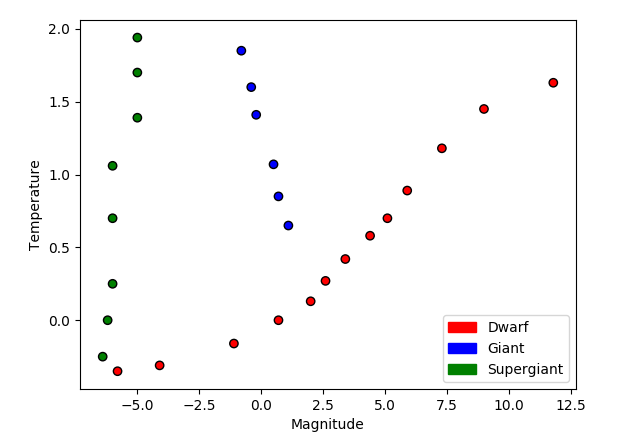
\includegraphics[width=.5\textwidth]{images/star.png}
\end{center}

Please implement the following classifiers in the \verb|SoftmaxRegression| and \verb|KNNClassifier| classes:

\begin{enumerate}[label=\alph*)]

\item \textbf{A multi-class logistic regression classifier} using the softmax activation function, which you investigated in Problem 2. In your implementation of gradient descent, \textbf{make sure to include a bias term and use L2 regularization} with regularization parameter $\lambda = 0.001$. Limit the number of iterations of gradient descent to 200,000, and set the learning rate to be $\eta = 0.001$.

\item \textbf{Another multi-class logistic regression classifier} with feature map $\phi(\boldx) = [\ln (x_1 + 10), x_2^2]^\top$, where $x_1$ and $x_2$ represent the values for magnitude and temperature, respectively.

\item \textbf{A kNN classifier} in which you classify based on the $k = 1$ and $k = 5$ nearest neighbors and the following distance function: $$dist(star_1, star_2) = (mag_1 - mag_2)^2/9 + (temp_1 - temp_2)^2$$
where nearest neighbors are those with the smallest distances from a given point.

  Note 1: When there are more than two labels, no label may have the
  majority of neighbors.  Use the label that has the most votes among
  the neighbors as the choice of label. 

  Note 2: The grid of points for which you are making predictions
  should be interpreted as our test space.  Thus, it is not necessary
  to make a test point that happens to be on top of a training point
  ignore itself when selecting neighbors.

\end{enumerate}

After implementing the above classifiers, complete the following exercises:

\begin{enumerate}
    \item Plot the decision boundaries generated by each classifier for the dataset. Include them in your PDF. 
    Identify the similarities and differences among the classifiers. What explains the differences---in particular, which aspects or properties of each model dictate the shape of its decision boundary? 
    
    \item 
    
    Consider a star with Magnitude 3 and Temperature -2. To which class does each classifier assign this star? Report the classification probabilities of this star for each model. 
    
    Interpret how each model makes its classification decision. What are the pros and cons of each interpretation? What else should we, the modelers, be aware of when making predictions on a test point ``far" from our training data? \textbf{Your response should no be longer than 5 sentences.}
\end{enumerate}
\end{problem}
\pagebreak
\textbf{Problem 3 Solution:}\\
\begin{enumerate}
    \item Softmax Regressions:\\
     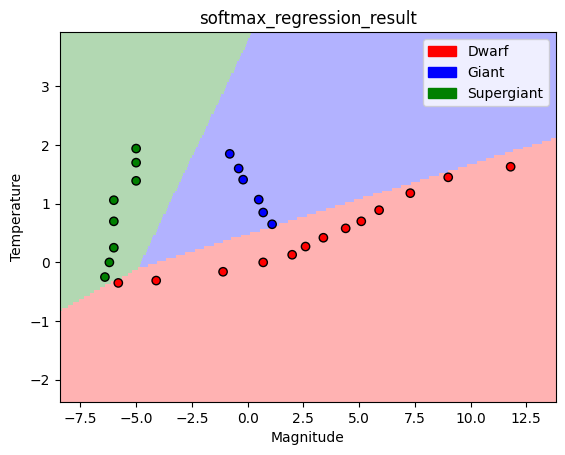
\includegraphics[scale=0.4]{hw2/images/softmax_regression.png}
     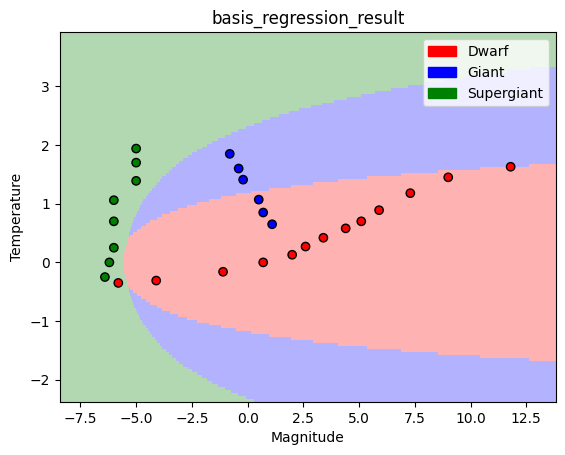
\includegraphics[scale=0.4]{hw2/images/basis_regression.png}\\
     KNN Regressions:\\
     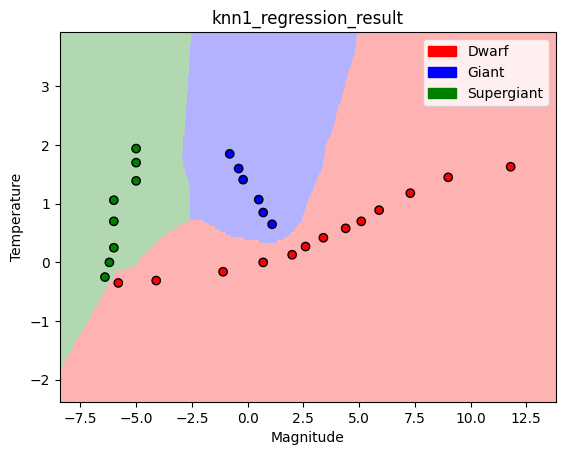
\includegraphics[scale=0.4]{hw2/images/knn1_regression.png}
     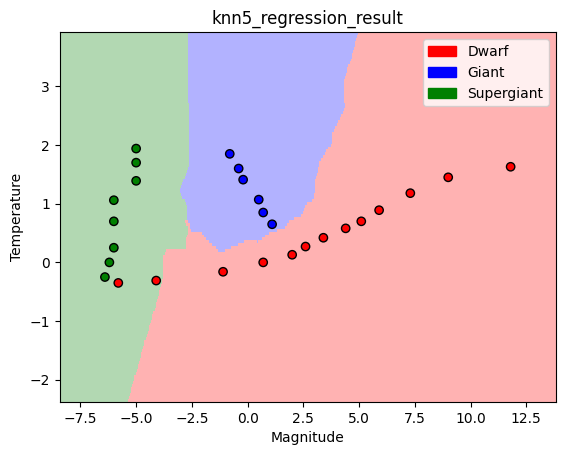
\includegraphics[scale=0.4]{hw2/images/knn5_regression.png}\\
     \\
     Looking at all of these graphs we can clearly see that each type of regression uses a different decision boundary. The standard softmax regression uses all linear decision boundaries because the data has not been transformed. From the plot, we can see that because of the linear boundaries, we cannot capture every point exactly, but overall the regression does a very good job classifying the stars. The softmax regression with the feature map (basis regression) uses quadratic looking decision boundaries. This is a result of the log and quadratic data transformation we used. There is no longer a linear term which is why the boundaries cannot be linear. This regression does not do nearly as good of a job classifying the data as in the standard softmax regression. Lastly, both of the KNN regressions have varying decision boundaries because all of the classifications are made from the points around them. Becauase of the flexibility in shape of the decision boundaries, they both do a good job of classifying the data. Furthermore we can see that when $k=1$ we are moving the boundary for every point - a clear sign of overfitting. \\
     \item
     I wrote some code which will identify which class each model predicts:\\
     \\
     \textbf{Softmax model:} predicts \textbf{Class 0} with probabilities: \\$[1.00000000e+00, 1.31778926e-28, 2.56768493e-40]$\\
     \\
     \textbf{Basis model:} predicts \textbf{Class 1} with probabilities:\\ $[0.03425432, 0.96455651, 0.00118917]$\\
     \\
     \textbf{KNN $k=1$ model:} predicts \textbf{Class 0}\\
     \textbf{KNN $k=5$ model:} predicts \textbf{Class 0}\\
     \\
     Both of the softmax models (the Softmax model and the Basis model) make their classification decisions based on classification probabilities meaning they see which class has the highest probability and assign that class overall. The KNN models, on the other hand, make their classification decisions based on the classification of the $k$ nearest training points - they choose whichever class is most common amongst its $k$ nearest neighbors, and, as a result, it does not use classification probabilities. The pros of the KNN models (and cons of the softmax models) are that the classification boundaries do not need to be as strict (ie they do not need to all be linear or quadratic) which can be beneficial. The cons, on the other hand, are that the choice of $k$ is very important (a bad choice can make our model either overfit or undefit), and KNN does not report classification probabilities so we are not able to clearly see the model's confidence in its predictions. \\
     In general, when making predictions on a test point "far" from our training data we should be aware that this point is farther away so the classification might be less accurate. This is particularly true for KNN models because we are classifying based on the points around so if the training point is not near other points then the classification of other points might not be helpful.
\end{enumerate}

%%%%%%%%%%%%%%%%%%%%%%%%%%%%%%%%%%%%%%%%%%%%%
% Problem 4
%%%%%%%%%%%%%%%%%%%%%%%%%%%%%%%%%%%%%%%%%%%%%

\begin{problem}[Impact Question: Understanding model-assisted decision making, uncertainty in classification and model interpretation in a high-stakes situation]

\textbf{Prompt:} A pharmaceutical drug company is conducting a clinical drug trial for a devastating disease for which conventional treatment is often ineffective. They want to estimate the effectiveness of a new drug on patients in order to obtain FDA approval and release the drug to the market. They approach you with the results of their clinical trial conducted on 100 patients with features and labels as follows:

Features = \{\textit{age, sex, height, blood pressure, drug administered?}\} \\
Label = \{\textit{Did the patient get cured?}\}

Since testing on a larger patient population is expensive for various reasons, they are interested in developing a machine learning model that will estimate the effectiveness of the drug. They provide you with covariate values of a single unseen patient for testing model performance. 

\begin{enumerate}
    \item You fit a logistic regression model on the 100 observations from the clinical trial and obtain the following coefficients which minimize the negative log likelihood. Let us call this model A:

    $p(y=1 | \mathbf{x}) = \sigma(0.2 + 0.8 *\text{\textit{drug administered?}} - 0.012 *\text{\textit{age}} + 0.45*\text{\textit{sex}} +  0.001*\text{\textit{height}} - 0.007*\text{\textit{blood pressure}})$

    Say you have a female (coded as 0) patient who is age 50, 168cm tall, blood pressure 140. What is the change in classification probability of the patient getting cured when they are administered the drug versus not (please show your work)?  Use your answer to formulate an interpretation of the value of $w_1$ -- the coefficient for \textit{drug administered?} -- for stakeholders in the drug company. The drug company wants you to answer whether or not you see evidence for the efficacy of their drug -- what would you say?

    \item The drug company wants to know you how confident you are that you have the right model, so you decide to sample the existing dataset with replacement to train 100 bootstrapped models. Upon testing these 100 models on the unseen patient, you find that the predictive interval of the classification probability is around $\pm 0.35$ averaged over the bootstrapped models. The drug company is concerned and asks you to check if you can choose alternative models that are more confident in their predictions:
    \begin{enumerate}
        \item You first try adding some interaction terms and train this new model B on the original dataset:

        $p(y=1 | \mathbf{x}) = \sigma(-2 + 5*\text{\textit{drug administered?}} + 2*\text{\textit{age}} - 3.3*\text{\textit{sex}} + 0.001*\text{\textit{height}} + 0.2*\text{\textit{blood pressure}} - 0.12*\text{\textit{age}}*\text{\textit{sex}} -0.34*\text{\textit{height}}*\text{\textit{sex}})$

        Bootstrapping model B 100 times gives you a new predictive interval of $\pm 0.1$ (averaged over bootstrapped models). Why might this be happening -- how would you explain this reduction in uncertainty in model B?

        \item Encouraged by the success of adding interaction terms, you add all possible combinations of interaction terms, repeat the exercise of bootstrapping 100 times and call this model C. This gives you a predictive interval of $\pm 0.39$ averaged over the bootstrapped models. Why might this be happening -- what is the source of this rise in uncertainty? What is a solution to reduce this comparatively large uncertainty, if you wished to keep all the new terms? 
        
        \item Which model (B or C, assuming you can reduce the predictive interval for model C) would you recommend to the drug company and why?
        
    \end{enumerate}

    \item Assume that the drug company has picked model B as their final model of choice because it seems the most confident in its predictions.
    \begin{enumerate}
        \item Suppose that the confidence interval of your estimate of $w_1$ ( coefficient for $drug$ $administered?$) is $\pm 6$. What would you recommend to a critically ill patient who is desperately seeking access to this new (and very expensive, not-covered-by-insurance) drug and why?
        \item The drug company has strong reasons to believe that the drug is indeed effective. What can the drug company do during the clinical trial to tighten the confidence interval of $w_1$?
    \end{enumerate}

\end{enumerate}
\end{problem}

\begin{framed}
\noindent\textbf{Problem 4} (cont.)\\
\begin{enumerate}
\item[3.] (Continued...)
     \begin{enumerate}
     \item[(c)] From prior clinical trials and modeling efforts, the drug company scientists strongly believe that the real value of $w_1$ is either 5 or 1. For now, you take this information as ground truth. In which scenario ($w_1=1$ or $w_1=5$) is it more costly to run the drug trial and demonstrate the effectiveness of the drug? Why?\\
        \textit{Hint:} In which case do you need your confidence intervals for the estimates of $w_1$ to be tighter, to demonstrate drug effectiveness?
        \item[(d)] How do you think we should make use of domain knowledge provided by our partners -- that the real value of $w_1$ is either 5 or 1 -- during model building? For example, would it be a good idea for us to simply fix the parameter $w_1$ to be 5 or 1?
    \end{enumerate}
\item[4.] Let us revisit the data collection process during the clinical trial and consider data collected from two recruitment protocols. In the first recruitment protocol, the drug company publicly advertised the development of this drug to a hospital, encouraging interested patients to sign up for the trial. Among an audience of 100, 50 patients agreed to be administered the drug and 50 choose to opt out and are observed in the study without administering the drug. In the second recruitment protocol, the company was referred 100 patients who have the disease and administered the drug to each patient randomly based on a coin flip. When you train model B on the first dataset, it has a high value of $w_1$ and a small confidence interval of this estimate. In contrast, when you train model B on the second dataset, you get a smaller value for $w_1$ with an equally small confidence interval. Which model would you trust to predict the probability of being cured from the disease given a randomly selected new patient from a Boston hospital? Why?
\textit{Hint:} What confounding factor might we have here?

\end{enumerate}
\end{framed}

\newpage
\textbf{Problem 4 Solution:}\\
\begin{enumerate}
    \item If the patient is administered the drug:\\
    $$p(y=1 | \mathbf{x}) = \sigma(0.2 + 0.8 - 0.012*50 +   0.001\cdot168 - 0.007\cdot140) = \sigma(-0.412) = 0.3984327$$
    If the patient is not administered the drug:\\
    $$p(y=1 | \mathbf{x}) = \sigma(0.2 - 0.012*50 +   0.001\cdot168 - 0.007\cdot140) = \sigma(-1.212) = 0.229347$$\\
    These results tell us that the change in probability that the patient is cured is $0.3984327 - 0.229347 = 0.1690857$. This change is not that substantial and in both cases it seems as though the patient would most likely not survive. Interestingly, however, the value of $w_1$ is $0.8$ which seems high especially when we compare it to the other coefficients. As a result, one might assume the coefficient has a large impact but in this case it doesn't seem to. Furthermore, we know that this small impact of the $w_1$ coefficient is a result of the behavior of the sigmoid function. The impact of the $0.8$ is very dependent on the other covariates. For example, if the patient had other factors that were very positively impacting her rate of survival then the drug might have had more of an impact. This means that in the worst case the drug has an impact of around $15\%$ and in the best case it has an impact of around $20\%$. \\
    As a result, in terms of evaluating the efficacy of their drug, I would say that this model definitely shows a correlation between a patient receiving a drug and the patient's rate of survival increasing, but we do not have enough evidence and the impact does not seem big enough to be able to determine if it is causal. \\
    \item
    \begin{enumerate}
        \item We might see this reduction in uncertainty in model B because we are making our model more complex so that it can fit the data better. Specifically, by adding these new interaction terms we are decreasing the bias of the model. This is very important because the model may no longer underfit the data quite as much. In addition, the variance is staying about the same which is why we see such an improvement - we are decreasing the bias without increasing the variance.
        \item In model C, we are increasing the complexity of our model too much which could be leading to overfitting. In model B we managed to decrease our bias without drastically increasing our variance which is why we saw a reduction in uncertainty - we were managing the bias / variance tradeoff well. However, in model C, as we get too complex our variance will substantially increase and our bias will decrease so we are not managing the tradeoff well. This is why our level of uncertainty rises.
        One way to reduce this comparatively large uncertainty while keeping all the new terms is to use Regularization - we can add either an L1 or L2 regularization term to our loss function in order to keep the coefficients low and decrease our variance.
        \item 
        I would recommend model B to the drug company because it is easier to interpret than model C. When we add too many terms to our model and make it too complex, it is difficult to understand exactly how each covariate is affecting the model. As a result, we will have more difficulty evaluating the model and extracting insights about the model. This is particularly important in a medical context. Just because a model predicts good outcomes for a drug, we should be sure we understand exactly why this is happening and other things that could impact survival before prescribing a drug that could potentially have many harmful effects. \\
    \end{enumerate}
    \item
    \begin{enumerate}
        \item I would not recommend this drug to the patient. This confidence interval is saying that within our $95\%$ confidence interval, there is a chance that the drug could actually have a negative affect on the patient. This means that the drug could actually make the critically ill patient sicker. As a result, especially if the drug is very expensive, I would not recommend that the patient test it out.
        \item If the drug company wants to tighten the confidence interval of $w_1$ then they can add more patients to their clinical trial. By increasing the number of patients they are increasing the data set size which decrease the variance in our model (as explained in question 1.3). With less variance, the drug company will be able to tighten the confidence interval of $w_1$ because there will be a smaller range of values that $w_1$ could take on. 
        \item It is more costly to run the drug trial to demonstrate the effectiveness of the drug when $w_1=1$. If we want to show that the drug is effective it cannot have a negative impact on the patient which means the value of $w_1$ cannot be negative. As a result, if $w_1=1$, the confidence interval must be much tighter because 1 is a lot smaller than 5 (it is closer to negative numbers).
        \item It would not be a good idea to fix the parameter $w_1$ because the aim of our model is to test whether or not the drug is effective. $w_1$ is the parameter that indicates the effectiveness so if we fix it then we would not know if the drug is effective. However, this domain knowledge can still be very beneficial because we can compare the values of $w_1$ generated by our model to their values as a sanity check. This might help us identify if our model is completely off base, or it might be the case that this domain knowledge is innacurate. \\
    \end{enumerate}
    \item 
    I would trust model B trained on the second data set rather than the first data set to predict the probability that this new random patient is cured when given the drug because the second data set is a randomly selected data set. In the first recruitment protocol, the patients themselves are able to choose whether or not they want to be in the trial. As a result, there could be several other factors amongst this group of people that impact the results of the trial. For example, patients that are more concerned about their health and will put more effort into taking care of themselves might be more willing to take the drug. As a result, the data could be skewed so that the people that opt in will have better outcomes. This is reflected in the model because $w_1$ is high for the first data set and much smaller for the second data set. The first data set seems to indicate that the drug is more effective but this could just be a result of the specific patients that decided to opt in. In this case, the willingness of patients to put in money / time to take care of themselves is a confounding factor in the first data set. However, in the second data set, because the patients are chosen randomly, this is no longer a confounding factor.   
    
    
    % the patients that are sicker and might have a worse case of the disease would be more likely to accept the drug because they are more desperate for a cure. Or, on the other hand, the people that want to invest more in their health might be more likely to Because the health of these patients are worse, they are more likely to die than the patients who have a milder version of disease which would mean the data could be skewed to indicate that the drug is not effective. This is proven when we learn that training model B on the first dataset yields a high value of $w_1$ and training it on the second dataset yields a smaller value for $w_1$. The first dataset seems to indicate that the drug is less effective but this could just be a result of the patients being sicker. In this case, the patient's health / level of severity of their disease is a confounding factor in the first data set. However, in the second data set, because the patients are chosen randomly, this is no longer a confounding factor.


\end{enumerate}
\newpage
%%%%%%%%%%%%%%%%%%%%%%%%%%%%%%%%%%%%%%%%%%%%%
% Name and Calibration
%%%%%%%%%%%%%%%%%%%%%%%%%%%%%%%%%%%%%%%%%%%%%
\subsection*{Name} Kara Siegel

\subsection*{Collaborators and Resources}
\textbf{Whom did you work with, and did you use any resources beyond cs181-textbook and your notes?}\\
Noah Covey, Natalie Melas-Kyriazi

\subsection*{Calibration}
\textbf{Approximately how long did this homework take you to complete (in hours)?}\\
25 hours



\end{document}
